%This is a Tex Version of NE 806 Homework Template
%
\documentclass{amsart}
\setlength{\textheight}{9in}
\setlength{\topmargin}{-0.25in}
\setlength{\textwidth}{7in}
\setlength{\evensidemargin}{-0.25in}
\setlength{\oddsidemargin}{-0.25in}
\usepackage{amsfonts}
\usepackage[utf8]{inputenc}
\usepackage[T1]{fontenc}
\usepackage{graphicx} 
\usepackage[export]{adjustbox}
\usepackage{fancyvrb}
% needed to include these graphics
%\graphicspath{{./Pictures/}}      % only in case you want to keep the pictures in a separate
                                  % subdirectory; also see the appropriate line below
\usepackage{caption}
\usepackage{subcaption}
\usepackage{float}
\usepackage{framed}
\newcounter{temp}
\theoremstyle{definition}
\newtheorem{Thm}{Theorem}
\newtheorem{Prob}{Problem}
\newtheorem*{Def}{Definition}
\newtheorem*{Ans}{Answer}
\newcommand{\dis}{\displaystyle}
\newcommand{\dlim}{\dis\lim}
\newcommand{\dsum}{\dis\sum}
\newcommand{\dint}{\dis\int}
\newcommand{\ddint}{\dint\!\!\dint}
\newcommand{\dddint}{\dint\!\!\dint\!\!\dint}
\newcommand{\dt}{\text{d}t}
\newcommand{\dA}{\text{d}A}
\newcommand{\dV}{\text{d}V}
\newcommand{\dx}{\text{d}x}
\newcommand{\dy}{\text{d}y}
\newcommand{\dz}{\text{d}z}
\newcommand{\dw}{\text{d}w}
\newcommand{\du}{\text{d}u}
\newcommand{\dv}{\text{d}v}
\newcommand{\ds}{\text{d}s}
\newcommand{\dr}{\text{d}r}
\newcommand{\dth}{\text{d}\theta}
\newcommand{\bbR}{\mathbb{R}}
\newcommand{\bbN}{\mathbb{N}}
\newcommand{\bbQ}{\mathbb{Q}}
\newcommand{\bbZ}{\mathbb{Z}}
\newcommand{\bbC}{\mathbb{C}}
\newcommand{\dd}[2]{\dfrac{\text{d}#1}{\text{d}#2}}
\newcommand{\dydx}{\dfrac{\text{d}y}{\text{d}x}}
\renewcommand{\labelenumi}{{\normalfont \arabic{enumi}.}}
\renewcommand{\labelenumii}{{\normalfont \alph{enumii}.}}
\renewcommand{\labelenumiii}{{\normalfont \roman{enumiii}.}}
\font \bggbf cmbx18 scaled \magstep2
\font \bgbf cmbx10 scaled \magstep2
\usepackage{fancyhdr}
\usepackage{lipsum}
\usepackage{amsmath}
\usepackage{empheq}
\newcommand*\widefbox[1]{\fbox{\hspace{2em}#1\hspace{2em}}}
% Clear the header and footer
\fancyhead{}
\fancyfoot{}
% Set the right side of the footer to be the page number
\rfoot{\thepage}
\fancyhf{}
\pagestyle{fancy}
\begin{document}
\LARGE{CIS 730: Principles of Artificial Intelligence}
 
\large
Machine Problem \#9
 
Solutions by: John Boyington
\newline
\bigskip


%%%%%%%%%%%%%%%%%%%%%%%%%%%%%%%%%%%%%%%%%%%%%%%%%%%%%%%%%%%%%%%%%%%%%%%%%%%%%%%%%%%%%%%%%%%%%%%%%%%%%%%%%%%%%%%%%%%%%%%%%%%
%                                                         PROBLEM 1
%%%%%%%%%%%%%%%%%%%%%%%%%%%%%%%%%%%%%%%%%%%%%%%%%%%%%%%%%%%%%%%%%%%%%%%%%%%%%%%%%%%%%%%%%%%%%%%%%%%%%%%%%%%%%%%%%%%%%%%%%%%

\textbf{Problem 1:}
\bigbreak

Object tracking is the task of recognizing an object and then being able to track the movement of that object within the robot's vision.
It is similar to the principle of object permanence in humans, where we learn that even though an object left sight for a moment, it still exists.
Keeping relative position under movement means that the machine is able to know where it is in space as it moves.
This challenge arises from the idea that when your velocity changes, the relative positions/velocities of other objects seem to change as well.
To solve this issue, the machine needs to have access to both its visual input stream, as well as some sensor that can tell its acceleration, velocity, etc.
This will allow it to correct the images that it is seeing mathematically and maintain knowledge of were it is.


%%%%%%%%%%%%%%%%%%%%%%%%%%%%%%%%%%%%%%%%%%%%%%%%%%%%%%%%%%%%%%%%%%%%%%%%%%%%%%%%%%%%%%%%%%%%%%%%%%%%%%%%%%%%%%%%%%%%%%%%%%%
%                                                         PROBLEM 2
%%%%%%%%%%%%%%%%%%%%%%%%%%%%%%%%%%%%%%%%%%%%%%%%%%%%%%%%%%%%%%%%%%%%%%%%%%%%%%%%%%%%%%%%%%%%%%%%%%%%%%%%%%%%%%%%%%%%%%%%%%%
\bigbreak
\textbf{Problem 2:}
\bigbreak





%%%%%%%%%%%%%%%%%%%%%%%%%%%%%%%%%%%%%%%%%%%%%%%%%%%%%%%%%%%%%%%%%%%%%%%%%%%%%%%%%%%%%%%%%%%%%%%%%%%%%%%%%%%%%%%%%%%%%%%%%%%
%                                                         PROBLEM 3
%%%%%%%%%%%%%%%%%%%%%%%%%%%%%%%%%%%%%%%%%%%%%%%%%%%%%%%%%%%%%%%%%%%%%%%%%%%%%%%%%%%%%%%%%%%%%%%%%%%%%%%%%%%%%%%%%%%%%%%%%%%
\bigbreak
\textbf{Problem 3:}
\bigbreak

The following is a screenshot from having completed the MLP demo in NeuroSolutions:

\begin{figure}[h!]
    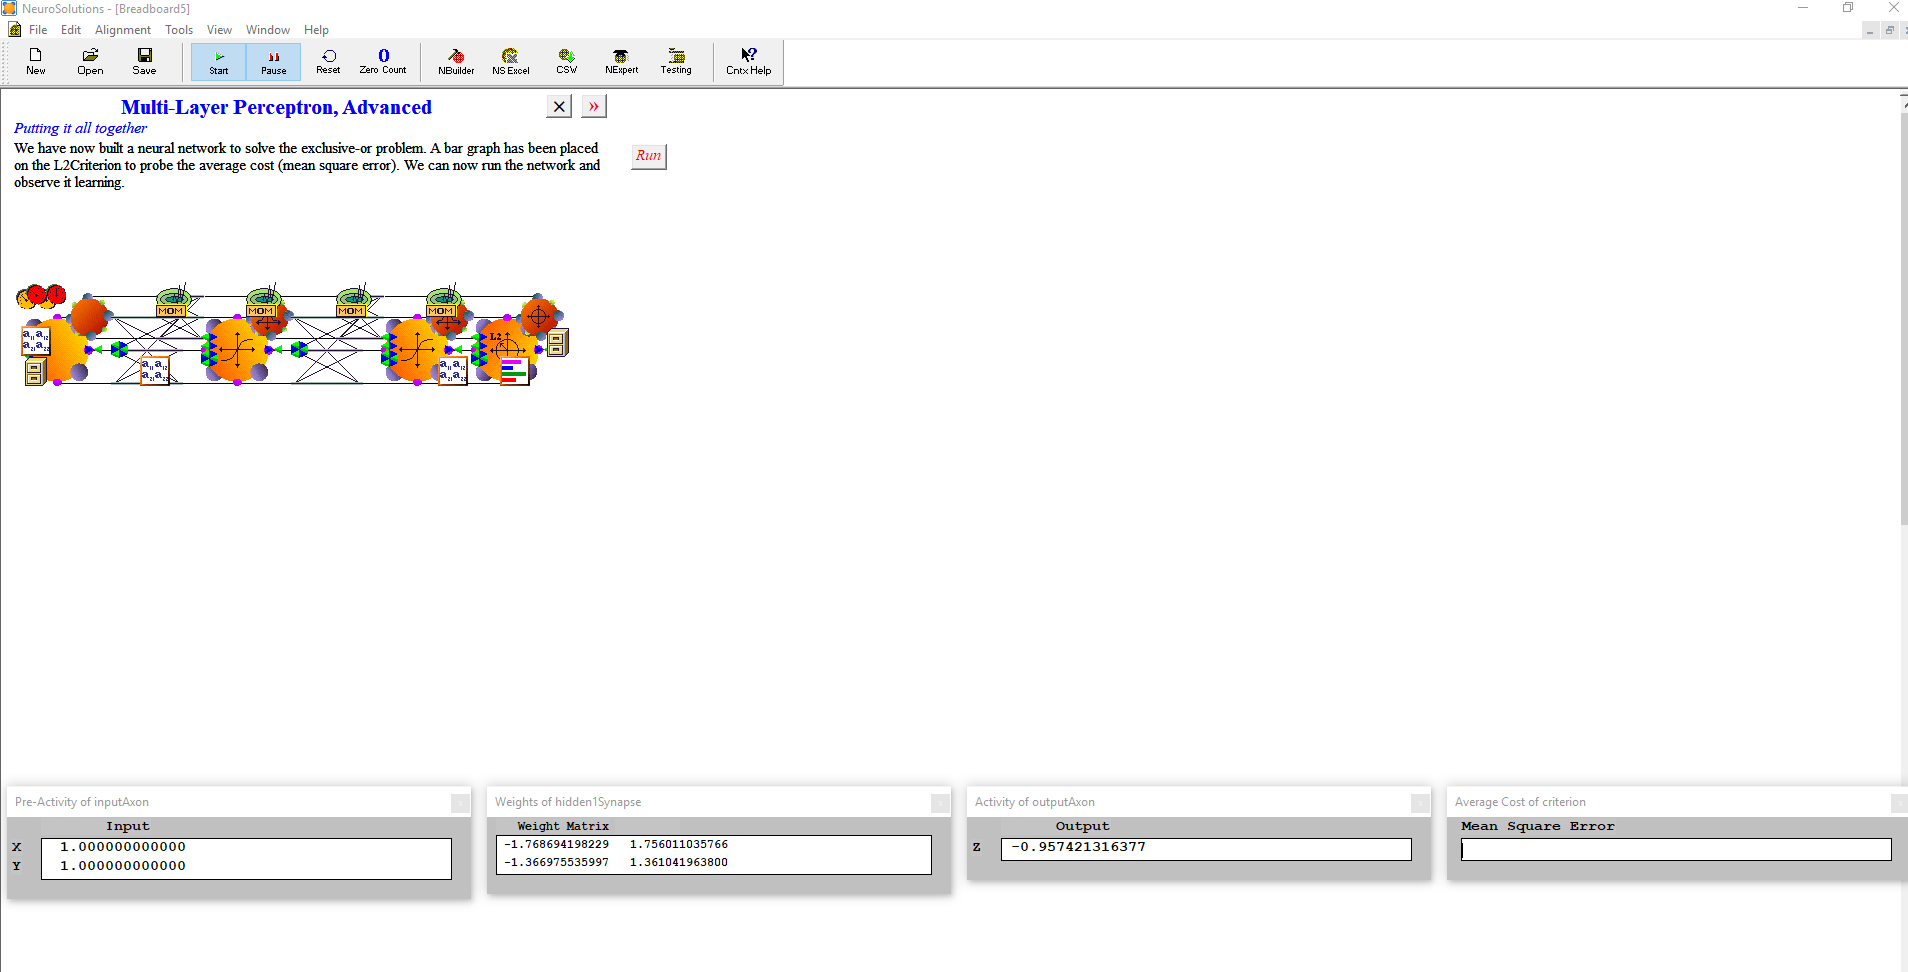
\includegraphics[width=0.9\linewidth]{mp9-3_0}
\end{figure}


The this screenshot is from training the robot control with the ARFF data:

\begin{figure}[h!]
    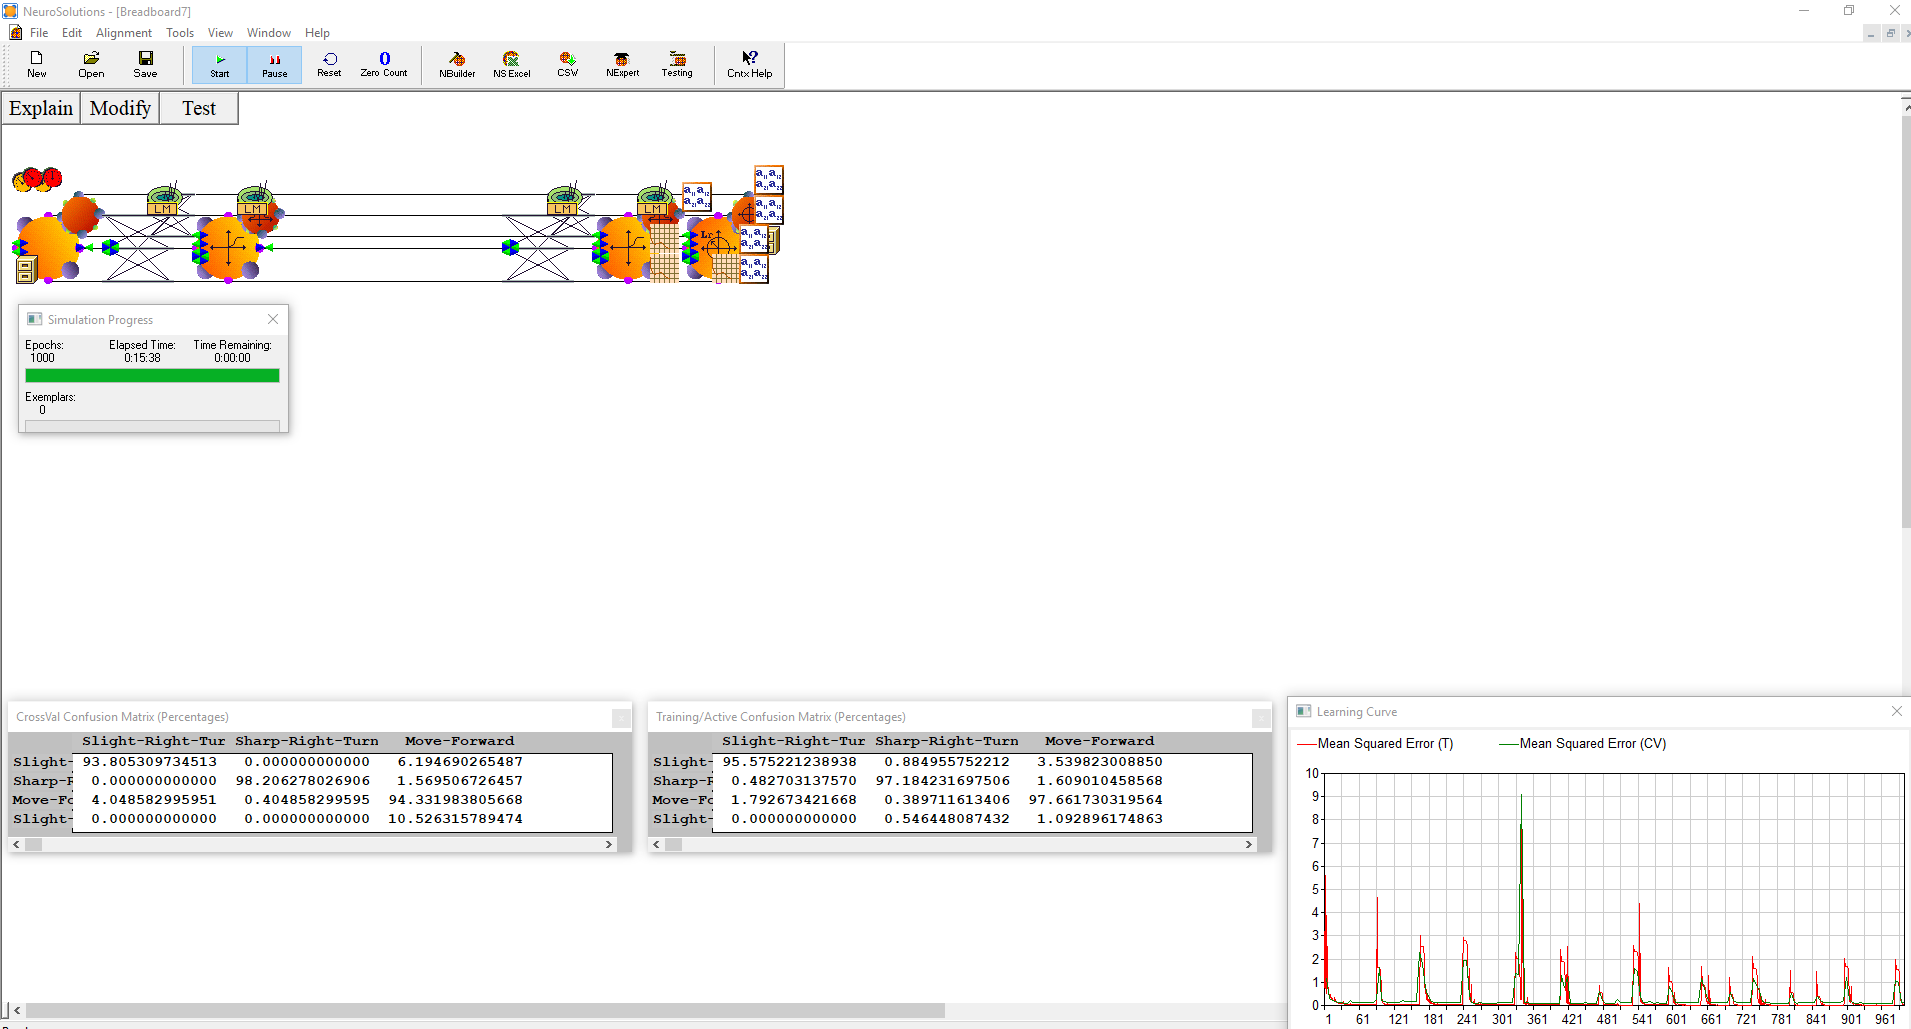
\includegraphics[width=0.9\linewidth]{mp9-3_1}
\end{figure}


%%%%%%%%%%%%%%%%%%%%%%%%%%%%%%%%%%%%%%%%%%%%%%%%%%%%%%%%%%%%%%%%%%%%%%%%%%%%%%%%%%%%%%%%%%%%%%%%%%%%%%%%%%%%%%%%%%%%%%%%%%%
%                                                         PROBLEM 4
%%%%%%%%%%%%%%%%%%%%%%%%%%%%%%%%%%%%%%%%%%%%%%%%%%%%%%%%%%%%%%%%%%%%%%%%%%%%%%%%%%%%%%%%%%%%%%%%%%%%%%%%%%%%%%%%%%%%%%%%%%%
\bigbreak
\textbf{Problem 4:}
\bigbreak

Located in {\tt MP9-4.zip} is the java files used in the ECJ tutorial4 and below is the output from running the tutorial:

\begin{verbatim}
| ECJ
| An evolutionary computation system (version 26)
| By Sean Luke
| Contributors: L. Panait, G. Balan, S. Paus, Z. Skolicki, R. Kicinger,
|               E. Popovici, K. Sullivan, J. Harrison, J. Bassett, R. Hubley,
|               A. Desai, A. Chircop, J. Compton, W. Haddon, S. Donnelly,
|               B. Jamil, J. Zelibor, E. Kangas, F. Abidi, H. Mooers,
|               J. O'Beirne, L. Manzoni, K. Talukder, S. McKay, J. McDermott
|               J. Zou, A. Rutherford, D. Freelan, E. Wei, E. Scott
| URL: http://cs.gmu.edu/~eclab/projects/ecj/
| Mail: ecj-help@cs.gmu.edu
|       (better: join ECJ-INTEREST at URL above)
| Date: July 1, 2017
| Current Java: 1.8.0_191 / OpenJDK 64-Bit Server VM-25.191-b12
| Required Minimum Java: 1.5


Threads:  breed/1 eval/1
Seed: 2059479409 
Job: 0
Setting up
Processing GP Types
Processing GP Node Constraints
Processing GP Function Sets
Processing GP Tree Constraints
Initializing Generation 0
Generation 1	Evaluations So Far 1024
Generation 2	Evaluations So Far 2048
Generation 3	Evaluations So Far 3072
Generation 4	Evaluations So Far 4096
Generation 5	Evaluations So Far 5120
Generation 6	Evaluations So Far 6144
Generation 7	Evaluations So Far 7168
Generation 8	Evaluations So Far 8192
Individual 553 of subpopulation 0 has an ideal fitness.
Total Evaluations 9216
\end{verbatim}


%%%%%%%%%%%%%%%%%%%%%%%%%%%%%%%%%%%%%%%%%%%%%%%%%%%%%%%%%%%%%%%%%%%%%%%%%%%%%%%%%%%%%%%%%%%%%%%%%%%%%%%%%%%%%%%%%%%%%%%%%%%
%                                                         PROBLEM 5
%%%%%%%%%%%%%%%%%%%%%%%%%%%%%%%%%%%%%%%%%%%%%%%%%%%%%%%%%%%%%%%%%%%%%%%%%%%%%%%%%%%%%%%%%%%%%%%%%%%%%%%%%%%%%%%%%%%%%%%%%%%
\bigbreak
\textbf{Problem 5:}
\bigbreak


I would have the signals from the sensors and motor control log output into a text file at a given time step (\~ .2s is probably good).
I would then use a file similar to my {\tt convert\_to\_arff.py} from problem 1 which would preprocess the data for use in something like WEKA.
This would produce a symbolic regressor, as the motor control takes the form of a class, not a numerical value.
The documentation mentions that the drive motors operate at a constant speed, so this is why it is classification (L or R motor Forward or Backward).
The ROS on the turtlebot would differ in the fact that there are different sensors than in the data we have above.
I would implement the neural network then, into the ROS and use it to drive the robot.


%%%%%%%%%%%%%%%%%%%%%%%%%%%%%%%%%%%%%%%%%%%%%%%%%%%%%%%%%%%%%%%%%%%%%%%%%%%%%%%%%%%%%%%%%%%%%%%%%%%%%%%%%%%%%%%%%%%%%%%%%%%
\end{document}
